% A hexagon for memorizing trigonometric identities

\documentclass{article}

\usepackage{tikz}

\begin{document}
	\huge
	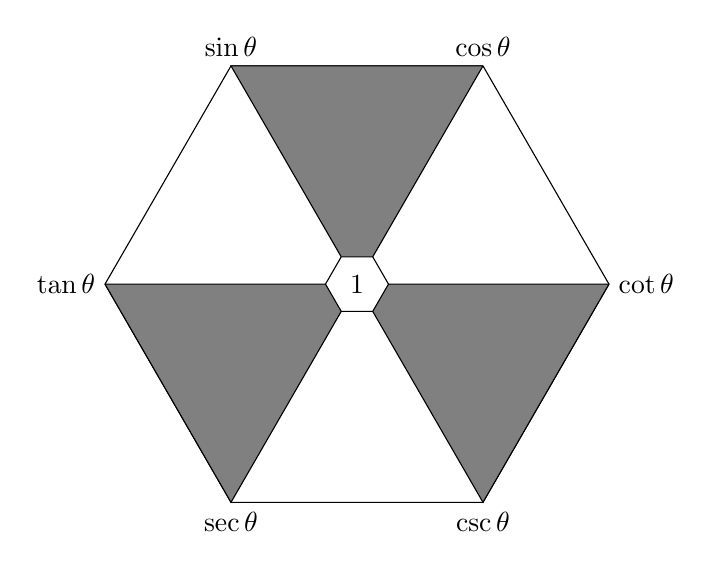
\begin{tikzpicture}[scale=4]
		% Radius of regular polygons
		\newdimen\R;
		\R=0.8cm;
		\coordinate (center) at (0,0);
		\draw (0:\R)
		\foreach \x in {60,120,...,360} { -- (\x:\R) }
		-- cycle (300:\R) node[below] {$\csc \theta$}
		-- cycle (240:\R) node[below] {$\sec \theta$}
		-- cycle (180:\R) node[left]  {$\tan \theta$}
		-- cycle (120:\R) node[above] {$\sin \theta$}
		-- cycle (60:\R)  node[above] {$\cos \theta$}
		-- cycle (0:\R)   node[right] {$\cot \theta$};
		\draw[fill=gray] { (60:\R) -- (120:\R) -- (center) -- (60:\R) };
		\draw[fill=gray] { (180:\R) -- (240:\R) -- (center) -- (180:\R) };
		\draw[fill=gray] { (0:\R) -- (300:\R) -- (center) -- (0:\R) };
		\R=0.1cm;
		\draw[fill=white] (0:\R)
		\foreach \x in {60,120,...,360} { -- (\x:\R) }
		-- cycle (center) node {$1$};
		% TODO
	\end{tikzpicture}
\end{document}
